\documentclass[12pt]{beamer}
%\documentclass[handout,xcolor=pdflatex,dvipsnames,table,12pt]{beamer}
\usepackage[latin1]{inputenc}
%\usepackage[T1]{fontenc}
\usepackage{amsmath} % for math AMS fonts
\usepackage{graphicx} % to include figures
\usepackage{subfigure} % to have figures in figures
\usepackage{multimedia} % to include movies
\usepackage{listings} % to display code
\usepackage{colortbl} % colored tables
\usepackage[latin1]{inputenc} % support for accented letters, etc.
\usepackage{amsthm}
\usepackage{hyperref}
\usepackage{ulem}
\usepackage{booktabs}
\usepackage{tikz}
\usepackage{mathtools}

\usetheme{Warsaw}
\setbeamercovered{invisible}

\title[Introduction to Cryptography]{Secure Multiparty Computation}
\author{Christian Mann -- christian-mann@utulsa.edu}
\institute{University of Tulsa\\
Tulsa, Oklahoma 74104}
\date{\today}

\logo{
\includegraphics[height=1.5cm]{pictures/SFSLogoMain}}

\begin{document}

\lstset{
language=python,                % choose the language of the code
%basicstyle=\footnotesize,       % the size of the fonts that are used for the code
%numbers=left,                   % where to put the line-numbers
%numberstyle=\footnotesize,      % the size of the fonts that are used for the line-numbers
%stepnumber=2,                   % the step between two line-numbers. If it's 1 each line will be numbered
%%umbersep=5pt,                  % how far the line-numbers are from the code
%backgroundcolor=\color{white},  % choose the background color. You must add \usepackage{color}
showspaces=false,               % show spaces adding particular underscores
showstringspaces=false,         % underline spaces within strings
showtabs=false,                 % show tabs within strings adding particular underscores
%%frame=single,	                % adds a frame around the code
tabsize=4,	                % sets default tabsize to 2 spaces
%%captionpos=b,                   % sets the caption-position to bottom
%%breaklines=true,                % sets automatic line breaking
%%breakatwhitespace=false,        % sets if automatic breaks should only happen at whitespace
%%title=\lstname,                 % show the filename of files included with \lstinputlisting; also try caption instead of title
%escapeinside={\%*}{*)}          % if you want to add a comment within your code
%morekeywords={*,...}            % if you want to add more keywords to the set
}

\newtheorem{mydef}{Definition}


\begin{frame}
\titlepage
\end{frame}


% no outline

% note, you should have three sections maximum.  two is good.  subsubsections are evil.
% new slides begin with teh \begin{frame} and end with \end{frame}

\iffalse
Secure Multiparty Computation -- definition/goal
Oblivious Transfer
	Rabin (quadratic)
	1-2 (RSA)
Yao's Millionaire Problem
Yao's Garbled Circuits
Secret Sharing
Mental Poker
Zero-Knowledge Proofs
\fi

\begin{frame}{Secure Multiparty Computation}
	\begin{block}{Definition}
		Methods for parties to jointly compute a function over their inputs
		while keeping those inputs private.
	\end{block}

	\begin{block}{Problem}
		In an MPC, a given number of participants, $p_1, p_2, ..., p_N$, each have
		private data, respectively $d_1, d_2, ..., d_N$. Participants want to compute
		the value of a public function on that private data: $F(d_1, d_2, ...,
		d_N)$
		while keeping their own inputs secret.
	\end{block}
\end{frame}

\begin{frame}{Secure Multiparty Computation}
	\begin{block}{Properties}
		\begin{description}
			\item[Input Privacy:] No information about the private data should
				be revealed, apart from the function output.
			\item[Correctness:] The function should compute the correct result,
				even in case of colluding malicious entities.
		\end{description}
	\end{block}

	\begin{alertblock}{Threat Model}
		Generally, we define our threat to be actors who are \textbf{trusted but
		curious}; they perform the protocol correctly, but try to infer
		extra information.
	\end{alertblock}
\end{frame}

\begin{frame}{Oblivious Transfer Protocol}
	\begin{block}{Idea}
		\begin{itemize}
			\item Sender has two messages $m_0, m_1$
			\item Receiver has bit $b$
			\item Receiver should learn $m_b$ but not $m_{1-b}$
		\end{itemize}
	\end{block}

	\begin{block}{Why is this useful?}
		The receiver (generally) has the opportunity to choose bit $b$; the
		server still has no knowledge of $b$
	\end{block}
\end{frame}

%\begin{frame}{Oblivious Transfer Protocol}{Details}
%	\[
%	\begin{array}{lllll}
%		m_0, m_1 & & & \\
%		d & N, e & \rightarrow & & N, e \\
%		& x_0, x_1 & \rightarrow & & x_0, x_1 \\
%		& & & k, b & \\
%		& v & \leftarrow & & v = (x_b + k^e) \\
%		\begin{array}{ll}
%			k_0 = (v-x_0)^d \\
%			k_1 = (v-x_1)^d
%		\end{array} & & & \\
%		& \begin{array}{ll}
%			m_0' = m_0 + k_0 \\
%			m_1' = m_1 + k_1
%		\end{array} & \rightarrow & & m_0', m_1' \\
%		& & & m_b = m_b' - k &
%	\end{array}
%	\]
%\end{frame}

\begin{frame}{Oblivious Transfer Protocol}{Details}
	\begin{itemize}
		\item Alice has two messages $m_0, m_1$; wants to send one to Bob.
		\item Alice generates an RSA key pair $(N, e, d)$.
		\item Alice generates two random values $x_0, x_1$.
		\item Bob chooses $b = 0$ or $b = 1$, selects $x_b$.
		\item Bob generates random $k$ and blinds $x_b$ by sending $v = (x_b +
			k^e) \mod N$
		\item Alice generates $k_0 = (v - x_0)^d$, and $k_1$. Either
			$k_0=k$ or $k_1=k$.
		\item Alice sends $m_0' = m_0 + k_0$ and $m_1'$ the same way.
		\item Bob knows either $k_0$ or $k_1$, and decrypts $m_0$ or $m_1$
			accordingly.
	\end{itemize}
\end{frame}

\begin{frame}{Rabin's OTP}
	\begin{block}{Probabilistic Transmission}
		The receiver has a $1/2$ chance of learning the message. This is
		equivalent to the given definition of OTP.
	\end{block}

	\begin{block}{Hard Problem}
		\centering
		Quadratic Residuosity! \small\textsuperscript{(Is anyone surprised?)}
	\end{block}

	\begin{itemize}
		\item Alice sends $N, e, m^e$
		\item Bob picks random $x$ and sends $x^2$ to Alice.
		\item Alice sends $y$, the square root of $x^2$, to Bob.
		\item If $x = y$, then Bob can factor $N$ and learn $m$.
	\end{itemize}
\end{frame}

\begin{frame}{Yao's Millionaire Problem}
	\begin{block}{Idea}
		Two millionaires want to know who has more money (or income) between them.
		\[ x \geq y \]
	\end{block}

	\begin{block}{Solution}
		Andrew Yao proposed a solution that was exponential in space and time.
		Since then, it has improved to $O(d^2)$, where each $x,y < 2^d$.
	\end{block}
\end{frame}

\begin{frame}{Yao's Garbled Circuits}
	\begin{block}{Idea}
		Secure computation of arbitrary functions via circuit evaluation. One
		player's input is ``compiled into'' the circuit; the other's is added.
	\end{block}

	\begin{exampleblock}{}
		Yes, this is very similar to homomorphic function evaluation
	\end{exampleblock}
\end{frame}

\begin{frame}{Yao's Garbled Circuits}
	\centering
	\begin{block}{Idea}
		Express a truth-value on each wire as a pair of keys. Gates are then
		functions from keys to keys.
	\end{block}

	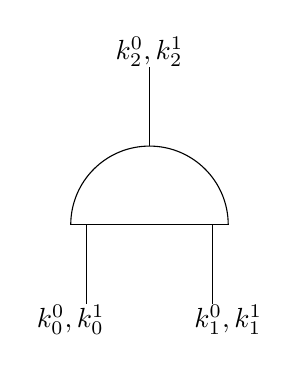
\begin{tikzpicture}
		\node (k0) at (0,-0.2) {$k_0^0, k_0^1$};
		\node (k1) at (2,-0.2) {$k_1^0, k_1^1$};
		\node (k2) at (1,3.2) {$k_2^0, k_2^1$};

		\draw (0.2, 0) -- (0.2, 1);
		\draw (1.8, 0) -- (1.8, 1);
		\draw (1, 2) -- (1, 3);

		\draw (0,1) arc (180:0:1);
		\draw (2,1) -- (0,1);
	\end{tikzpicture}
\end{frame}

\begin{frame}{Yao's Garbled Circuits}

	\begin{columns}
		\column{.5\textwidth}
		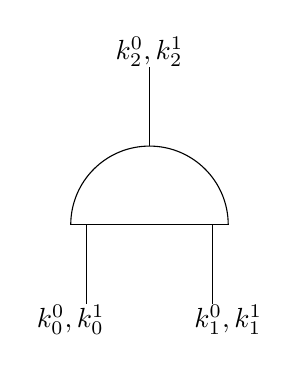
\begin{tikzpicture}
			\node (k0) at (0,-0.2) {$k_0^0, k_0^1$};
			\node (k1) at (2,-0.2) {$k_1^0, k_1^1$};
			\node (k2) at (1,3.2) {$k_2^0, k_2^1$};

			\draw (0.2, 0) -- (0.2, 1);
			\draw (1.8, 0) -- (1.8, 1);
			\draw (1, 2) -- (1, 3);

			\draw (0,1) arc (180:0:1);
			\draw (2,1) -- (0,1);
		\end{tikzpicture}

		\column{.5\textwidth}
		\textbf{Truth Table} \\
		\begin{tabular}{cc|c}
			0 & 0 & 0 \\
			0 & 1 & 0 \\
			1 & 0 & 0 \\
			1 & 1 & 1
		\end{tabular}

		\textbf{Circuit Description} \\
		\begin{tabular}{c}
			$E_{k_0^0}(E_{k_1^0}(k_2^0))$ \\
			$E_{k_0^0}(E_{k_1^1}(k_2^0))$ \\
			$E_{k_0^1}(E_{k_1^0}(k_2^0))$ \\
			$E_{k_0^1}(E_{k_1^1}(k_2^1))$
		\end{tabular}
	\end{columns}
\end{frame}

\begin{frame}{Yao's Garbled Circuits}{Input/Output}
	Alice's input is compiled into the circuit.

	The keys corresponding to Bob's input are obtained via OTP.

	\[ (k_0^0, k_0^1) \rightarrow k_0^b \]

	When Bob finishes evaluating the circuit, he sends the result to Alice, who
	decodes it to a value.

	\begin{block}{}
		Remember: our adversary is the \textbf{trusted but curious} participant.
	\end{block}
\end{frame}

\begin{frame}{Secure Computation with Active Adversaries}
	\begin{block}{Collusion}
		With enough collusion, almost all bets are off; e.g. \textit{mean}
		function with $n-1$ colluding players
	\end{block}

	\begin{block}{}
		There exist protocols that guarantee good results as long as no more
		than $k$ players collude (sometimes called ``corrupted'')
	\end{block}
\end{frame}

\begin{frame}{Secret Sharing Schemes}
	\begin{block}{Goal}
		Split a secret into $n$ parts s.t. any $t$ shares can combine and
		reconstruct the original secret
	\end{block}

	\begin{block}{Ideas}
		\begin{itemize}
			\pause
			\item XOR Encryption
			\item Shamir's Secret Sharing (polynomials)
			\item Plane Intersection
			\item Chinese Remainder Theorem
		\end{itemize}
	\end{block}
\end{frame}

\begin{frame}{XOR Secret Sharing}
	Only supports $n$-of-$n$ sharing. To split a $k$-digit secret:
	\begin{itemize}
		\item Create $n-1$ random bitstrings $k_0, k_1, ..., k_{n-1}$
		\item Let $k_n = k \oplus k_0 \oplus k_1 \oplus ... \oplus k_{n-1}$
		\item Then $k$ is the XOR of all key shards
		\item Even with $n-1$ shards, there is no knowledge of $k$
	\end{itemize}
\end{frame}

\begin{frame}{Shamir's Secret Sharing}
	\begin{block}{Theorem}
		You can fit a unique polynomial of degree $t-1$ to any set of $t$ points
		on the curve. Two points define a line, three points define a parabola,
		etc.
	\end{block}

	\begin{itemize}
		\item Create a polynomial of degree $t-1$ with secret as first
			coefficient
		\item Generate $n$ points on the curve, give those out
		\item With $t$ points you can reconstruct the equation
	\end{itemize}

	\begin{alertblock}{}
		Note: This is usually performed over a finite field e.g. $\mathbb{F}_p$.
	\end{alertblock}
\end{frame}

\begin{frame}{Blakley's Scheme (Plane Intersection)}
	\begin{block}{Theorem}
		Two nonparallel lines intersect at a point. Any $n$ nonparallel
		$(n-1)$-dimensional hyperplanes intersect at exactly
		one point.
	\end{block}

	\begin{itemize}
		\item Encode the secret as a point in $t$-dimensional space
		\item Generate $n$ nonparallel hyperplanes passing through that point
	\end{itemize}

	\begin{alertblock}{}
		Each participant does have enough information to narrow the solution
		down quite a bit. This, too, is often done over a finite field.
	\end{alertblock}

	\centering
	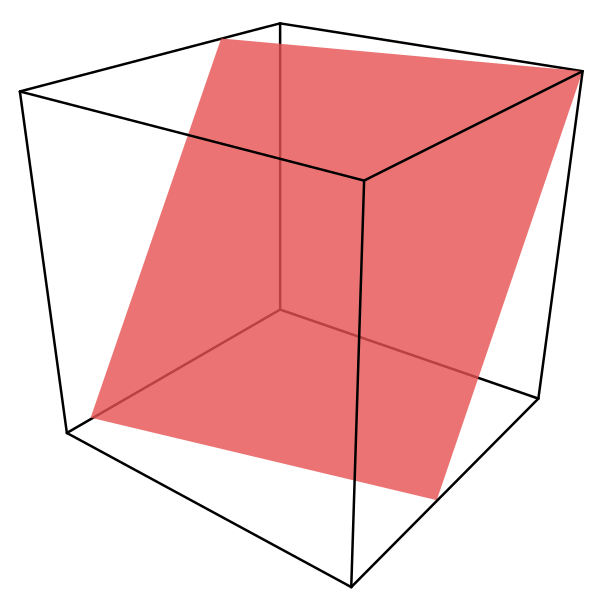
\includegraphics[width=0.1\textwidth]{./pictures/ss_planes1}
	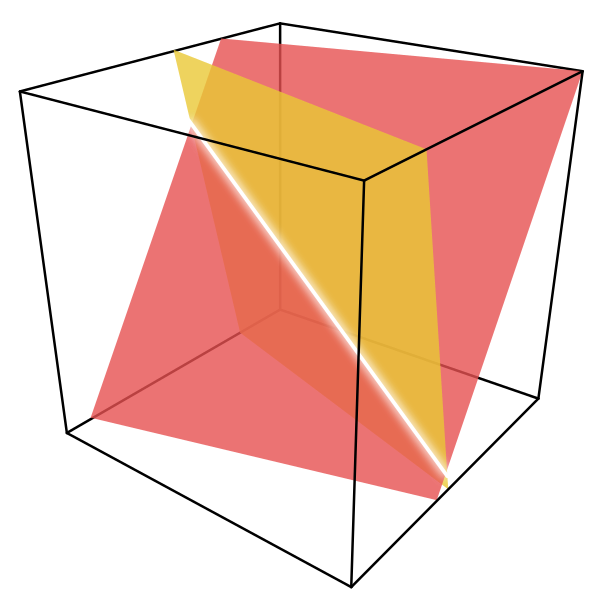
\includegraphics[width=0.1\textwidth]{./pictures/ss_planes2}
	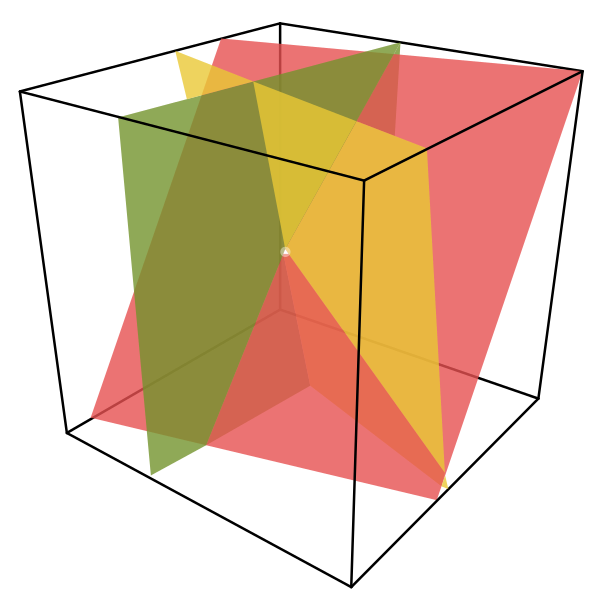
\includegraphics[width=0.1\textwidth]{./pictures/ss_planes3}
\end{frame}

\begin{frame}{Chinese Remainder Theorem}
	\begin{block}{Theorem}
		A number is uniquely defined modulo $p_1p_2...p_n$ by a set of $n$
		equivalences modulo each $p_i$
	\end{block}

	\begin{itemize}
		\item Encode secret as number $S$
		\item Choose a set of prime numbers $p_1, ..., p_n$
		\item $S$ should be larger than product of $t-1$ primes, but larger than
			product of $t$ primes
		\item Calculate each residue modulo $p_i$, distribute these
	\end{itemize}

	Once you have $t$ shares, you can compute $S$.
\end{frame}

\begin{frame}{Multiparty Computation (More Than 2)}
	Most MPC protocols make use of secret sharing.

	\begin{itemize}
		\item Each person splits their input among everyone
		\item The actors collectively evaluate the circuit
	\end{itemize}

	\begin{block}{}
		Some of these protocols can tolerate up to e.g. $n/3$ malicious actors
		or $n/2$ colluding actors.
	\end{block}
\end{frame}

\begin{frame}{Performance}{What did you really expect}
	\textbf{AES-128, 128-bit key, Two Party}
	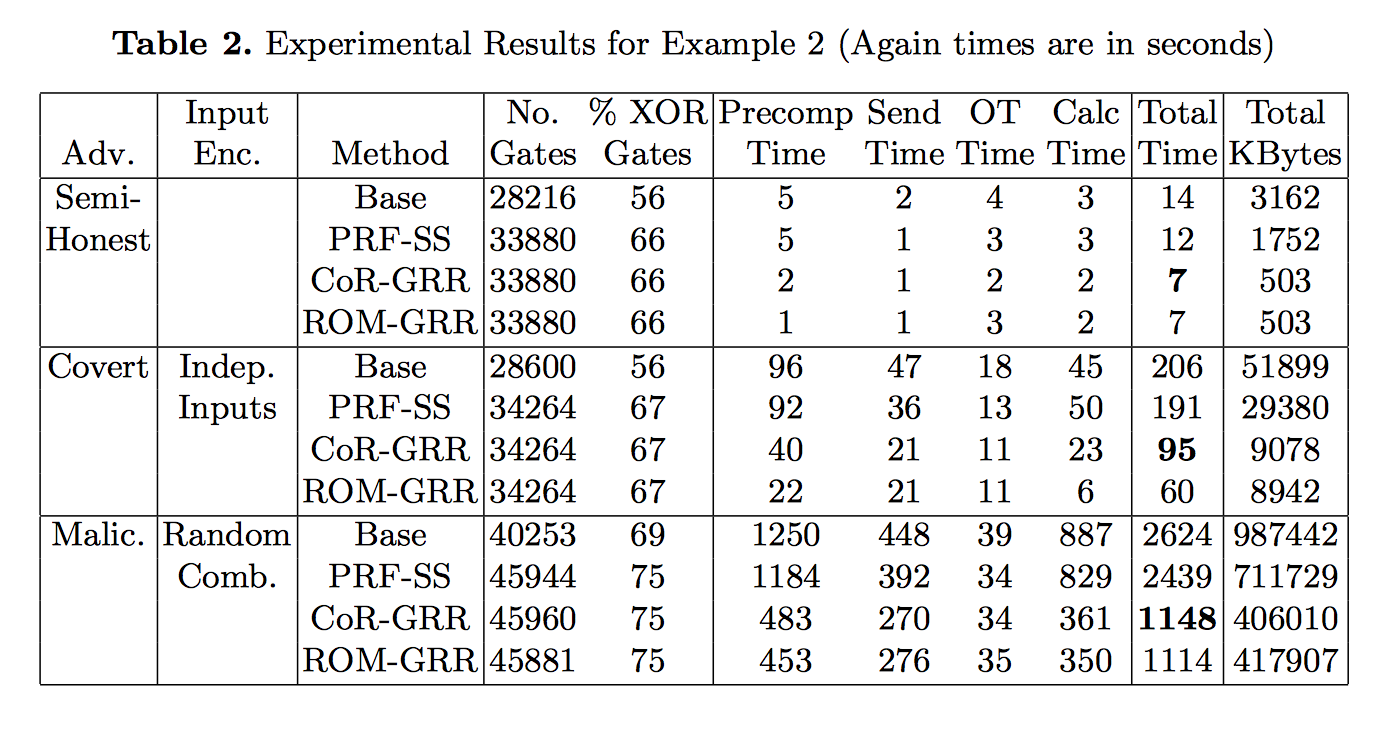
\includegraphics[width=\textwidth]{./pictures/smp-aes-performance1}
	\Tiny{
	B. Pinkas, T. Schneider, N. Smart, and S. Williams. ``Secure Two-party
	Computation is Practical''. In Advances in Cryptology--Asiacrypt, 2009.}
\end{frame}

\begin{frame}{Performance}{What did you really expect}
	\textbf{AES-128, 128-bit key, Multiparty}

	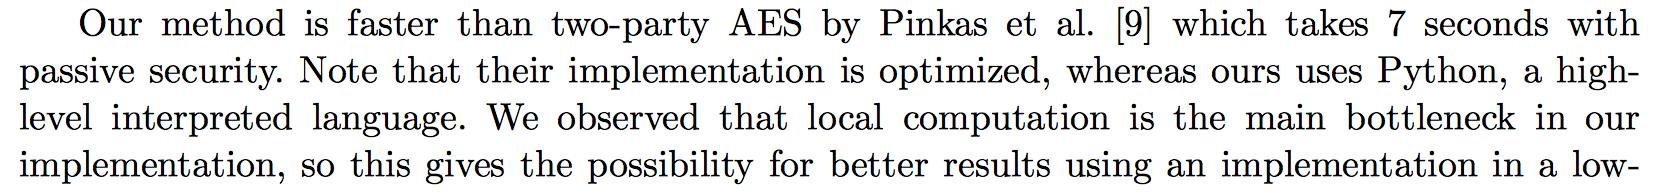
\includegraphics[width=\textwidth]{./pictures/smp-aes-2-performance1}

	\vspace{1em}
	\hrule
	\vspace{1em}

	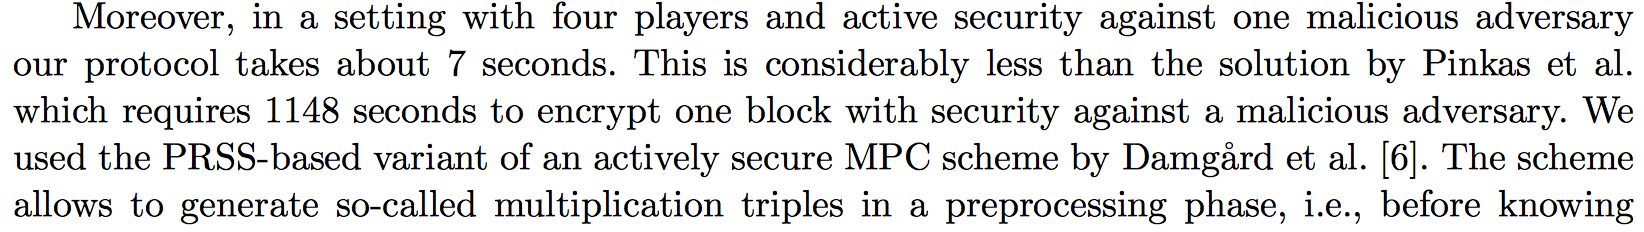
\includegraphics[width=\textwidth]{./pictures/smp-aes-2-performance2}
	
	\Tiny{
	Damg\o{a}rd, I., Keller, M.: ``Secure multiparty AES (full paper)''. IACR
	Cryptology ePrint Archive 2009:614 (2009)}
\end{frame}

\begin{frame}{Questions / Comments?}{We'll find out the answer together}
\end{frame}

\end{document}
